% !TeX root = RJwrapper.tex
\title{\href{https://CRAN.R-project.org/package=binGroup2}{binGroup2}: Statistical Tools for Infection Identification via Group Testing}


\author{by Christopher R. Bilder, Brianna D. Hitt, Brad J. Biggerstaff, Joshua M. Tebbs, and Christopher S. McMahan}

\maketitle

\abstract{%
Group testing is the process of testing items as an amalgamation, rather than separately, to determine the binary status for each item. Its use was especially important during the COVID-19 pandemic through testing specimens for SARS-CoV-2. The adoption of group testing for this and many other applications is because members of a negative testing group can be declared negative with potentially only one test. This subsequently leads to significant increases in laboratory testing capacity. Whenever a group testing algorithm is put into practice, it is critical for laboratories to understand the algorithm's operating characteristics, such as the expected number of tests. Our paper presents the \href{https://CRAN.R-project.org/package=binGroup2}{binGroup2} package that provides the statistical tools for this purpose. This R package is the first to address the identification aspect of group testing for a wide variety of algorithms. We illustrate its use through COVID-19 and chlamydia/gonorrhea applications of group testing.
}

\section{Introduction}

\noindent The COVID-19 pandemic showed the need for accessible, fast,
and reliable testing for severe acute respiratory syndrome coronavirus
2 (SARS-CoV-2) and for infections in general. To meet this need,
many laboratories turned to the use of group testing. Group testing---also 
known as pooled testing, specimen pooling, batch testing, and
bulk testing---involves combining portions of multiple specimens from
different individuals into a ``group'' and testing this group as
if it were a single specimen. If the group tests negative, all individuals
represented within it generally can be declared negative. Thus, for
a group of size 10, it takes only one test to determine whether all 10 individuals
are infection free, whereas it would take 10 tests if each specimen
was tested separately. Alternatively, if a group tests positive,
retesting in some form is needed to determine who is positive or negative
within the group. \citet{dorfman1943detection} proposed the original
retesting method that involved simply retesting each group member
separately using the remaining portions of their specimens. Since
this seminal paper, many other group testing algorithms have been
proposed. These algorithms are categorized into hierarchical and non-hierarchical
approaches corresponding to whether specimens are tested in non-overlapping
or overlapping groups, respectively, at each stage of the algorithm
(\citealt{hitt2019objective}).

A large number of research papers (see e.g. \citealt{abdalhamid2020assessment};
  \citealt{Hogan2020}; \citealt{barathidasan2022pooled}), articles
in the news media (see e.g. \citealt{ABCnews}; \citealt{NYTimesMandavilli};
\citealt{NYTimesAnthes}), and Emergency Use Authorizations given
by the US Food and Drug Administration (\citealt{LabCorp}; \citealt{Verily};
\citealt{Yale}) showed that group testing was one of the important
tools available to mitigate the crisis caused by COVID-19. Our new
\CRANpkg{binGroup2} package for the R software environment  provides
the statistical tools that researchers and laboratories need for group
testing. This package is available from the Comprehensive R Archive
Network (CRAN) at \url{https://CRAN.R-project.org/package=binGroup2}.
By its name, one can surmise that it is the second large-scale implementation
of the package. The \CRANpkg{binGroup} package (\citealt{Bilder2010b})
focused on estimation using the unique type of data that arises through
group testing. Its applications ranged from estimating an overall
infection prevalence to estimating a regression model for individual-specific
infection probabilities as a function of risk factors. \citet{Bilder2010b}
encouraged researchers to provide new functions so that there would
be one main package for group testing in R. This resulted in new functions
for estimation and a few functions focused on the identification aspect
of group testing (i.e., determine a positive/negative outcome for
each individual). Over time, these additions resulted in many different
syntax styles among functions, making use of the package inconsistent
and more difficult. The new \CRANpkg{binGroup2} package was created to
unify function syntax and, most importantly, to incorporate a new
suite of functions for identification. These new functions provide
the information that laboratories need to increase their testing capacity
to its fullest potential.

Our paper focuses on these identification functions of \CRANpkg{binGroup2}
because they represent the main new contribution of the package.
There are two other R packages on CRAN that also examine the identification
aspect of group testing but for different settings. First, the \pkg{gtcorr}
package (\citealt{gtcorr}; archived in 2022) examines hierarchical
and non-hierarchical algorithms for a homogeneous population when
there is a constant correlation among individuals within a group.
This package implements the work of \citet{lendle2012group} that
uses single-infection assays only. Second, the \CRANpkg{mMPA} package
(\citealt{mMPA}) examines three hierarchical algorithms, where two
are for homogeneous populations and one is for heterogeneous populations.
This package implements the work of \citet{tao2017improved} for single-infection
assays that return an additive count outcome (e.g., viral load) when
applied to a group. Both \pkg{gtcorr} and \CRANpkg{mMPA} are useful
for their specialized situations. Our package encompasses a total
of 27 different algorithms that include homogeneous/heterogeneous
populations and hierarchical/non-hierarchical algorithms. These algorithms
are constructed for the most common setting of a binary test response
(positive/negative) from independent individuals within a group. We
allow for the possibility of testing error and single or multiple-infection
assays. Our package implements the work of more than ten papers on
the identification aspect of group testing (e.g., \citealt{Kim2007};
\citealt{mcmahan2012two}; \citealt{houarray1}).

An outline of our paper is as follows. The next section  provides
a review of group testing algorithms that are commonly used by laboratories.
The third section discusses how to calculate important operating characteristics,
such as the expected number of tests, for a group testing algorithm
by using \CRANpkg{binGroup2}. This section also demonstrates how one
can choose the most efficient implementation of an algorithm. Finally,
we conclude with an  overview of changes to estimation functions
and future extensions of the package. Throughout our text,
we phrase our discussion in the context of testing humans for infectious
diseases. Applications of group testing for this purpose outside
of COVID-19 include testing for influenza (\citealt{van2012pooling}),
gonorrhea (\citealt{ando2020modified}), HIV (\citealt{kim2014pooled}),
and West Nile virus (\citealt{ARC}). The package can also be used
in a wide variety of other areas where group testing is implemented,
such as infectious disease testing for farm animals (\citealt{NVDC}),
detection of human exposure to pollutants (\citealt{thai2020analysis}),
determination of virus presence in insect carriers (\citealt{zhao2020thrips}),
development of new pharmaceuticals (\citealt{salzer2016screening}),
and security of computer networks (\citealt{thai2011group}).


\section[Algorithms]{Algorithms\label{sec:Algorithms}}

Laboratories select a group testing algorithm by examining 1) the
expected number of tests needed to make a positive/negative determination
for every individual, 2) the expected accuracy of the positive/negative
determinations, 3) the information available on individuals tested,
and 4) the ease of implementation. The \CRANpkg{binGroup2} package provides
computations needed to address 1) through 3), while laboratories need
to address 4) relative to their work environment. Overall, there is
not one group testing algorithm that is best for all situations, which
has resulted in many different hierarchical and non-hierarchical algorithms
being used in practice.

\subsection{Hierarchical algorithms}

Hierarchical group testing algorithms involve testing a group and
splitting its members into smaller, non-overlapping sub-groups for
retesting if the original group tests positive. These sub-groups are
split further whenever they test positive. If a group/sub-group tests
negative, its members are declared negative, so that no further testing
is performed upon them. Overall, testing can continue until each group
member is tested separately. 

A recent example of a hierarchical algorithm comes from \citet{lohse2020pooling}
to test for SARS-CoV-2 (see Figure \ref{fig:hierarchical-Lohse}).
Individuals were put into non-overlapping groups of size 30. If a
group tested positive, three non-overlapping groups of size 10 were
formed from its members. If one of these sub-groups tested positive,
each of its members were retested separately (i.e., individual testing).
This hierarchical algorithm is referred to as a three-stage algorithm
because three distinct stages are defined for it.

\begin{figure}
\begin{centering}
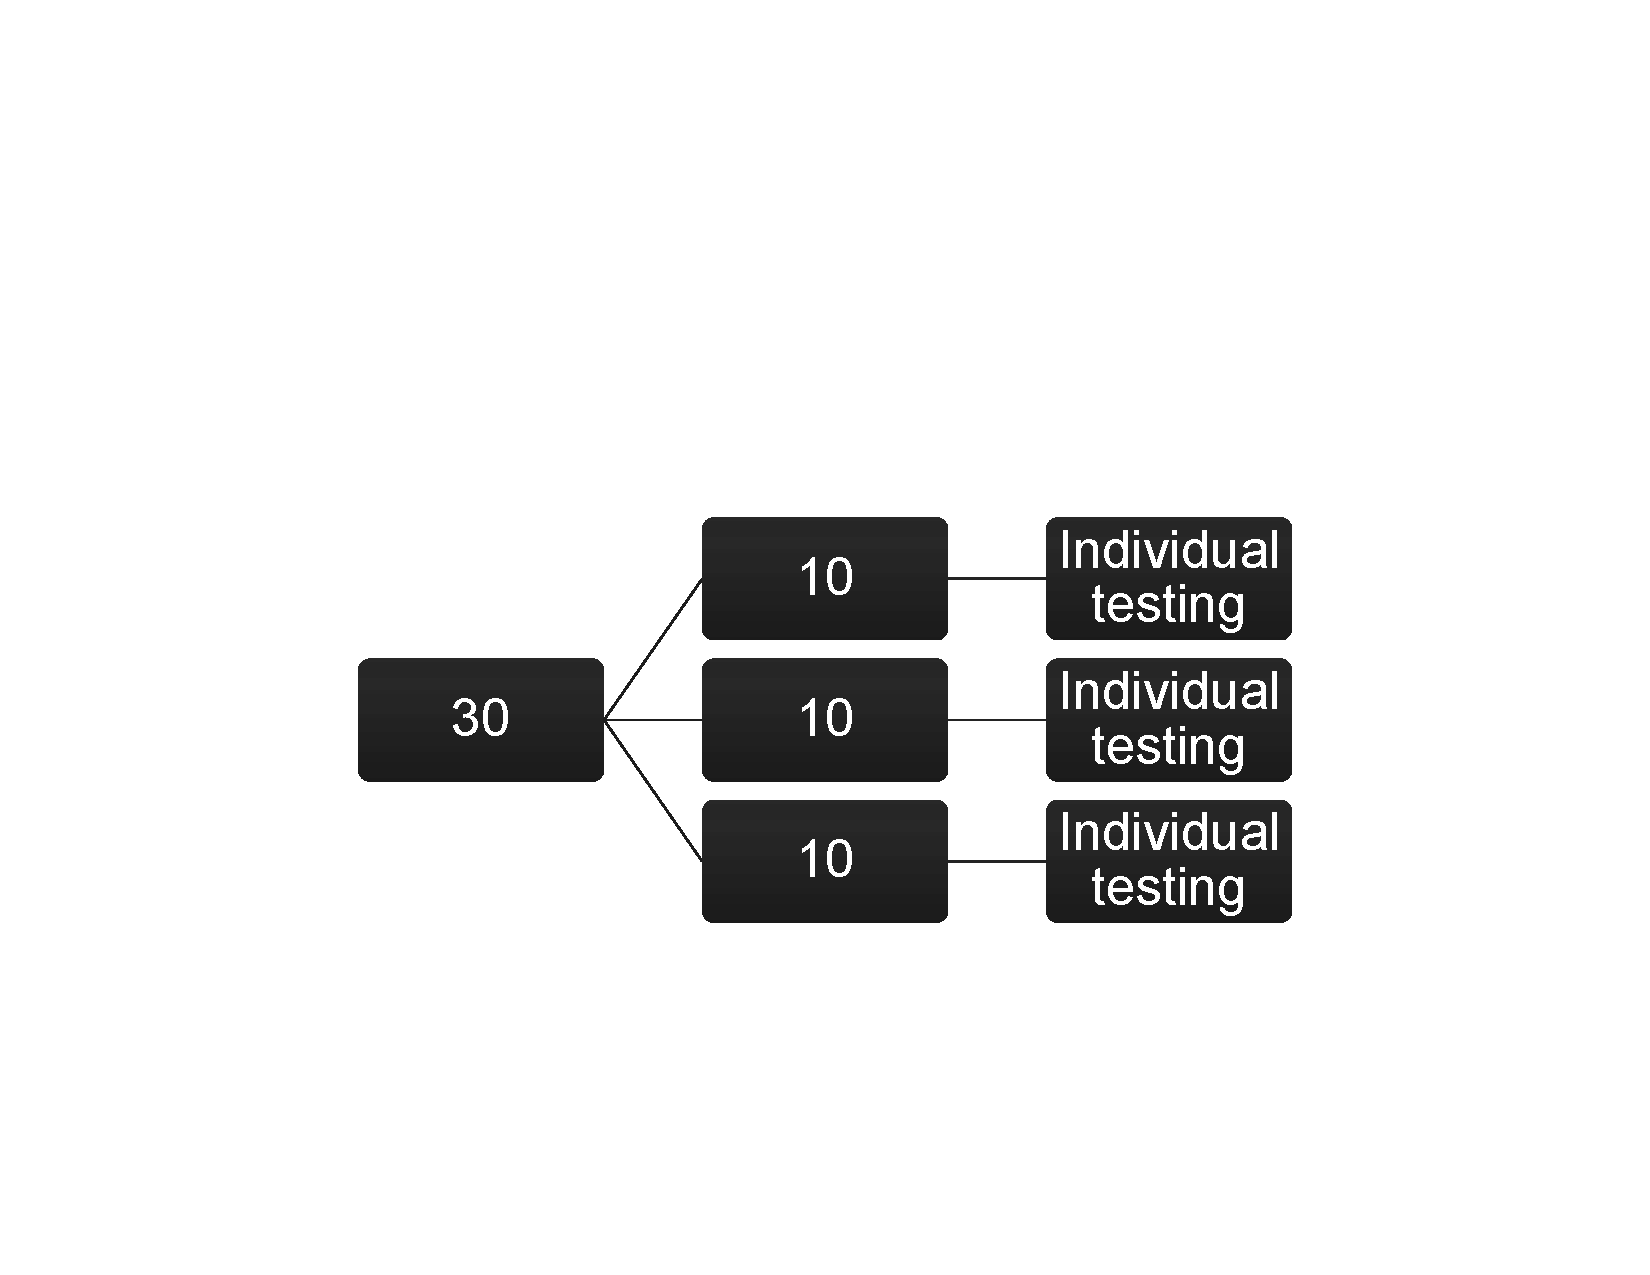
\includegraphics[scale=0.37]{figures/images_hier30-10-1BW.pdf}
\par\end{centering}
\caption{\label{fig:hierarchical-Lohse}The hierarchical testing algorithm
of \citet{lohse2020pooling}.}
\end{figure}

Hierarchical algorithms can have more or fewer stages than used by
\citet{lohse2020pooling}. For example, \citet{abdalhamid2020assessment}
used two stages for SARS-CoV-2 detection by testing in groups of size
5 and subsequently retesting each member of a positive group separately.
More than three stages are possible as well, but applications are
much rarer because of logistics, larger chance for error, and delay
in obtaining the positive/negative individual outcomes. With respect
to the last reason, this delay can be significant for nucleic acid
amplification tests which can take hours to complete. For example,
the Centers for Disease Control and Prevention's  assay to detect
SARS-CoV-2 takes approximately four hours to complete.

\subsection{Non-hierarchical algorithms}

Non-hierarchical algorithms were developed to minimize the number
of retests needed after an initial stage of testing. The most prominent
of these algorithms is referred to as array testing (also known as
matrix pooling). For this algorithm, specimens are arranged in a grid
(see Figure \ref{fig:array-1-1}). Groups are formed by row and by
column, and each of these groups are subsequently tested. Specimens 
that lie at the intersections of positive testing rows and
positive testing columns are retested separately in a second stage
to determine a positive/negative outcome for each of them. All other
specimens are declared negative. Because the accuracy of infectious
disease assays is not perfect, ambiguities may occur, resulting in
positive rows (columns) without any positive columns (rows). In those
situations, members of positive rows (columns) should be retested
separately (\citealt{Kim2007}). A recent example of an array testing
algorithm is the use of a $5\times5$ array by LabCorp for SARS-CoV-2
detection (\citealt{LabCorp}).

\begin{figure}
\begin{centering}
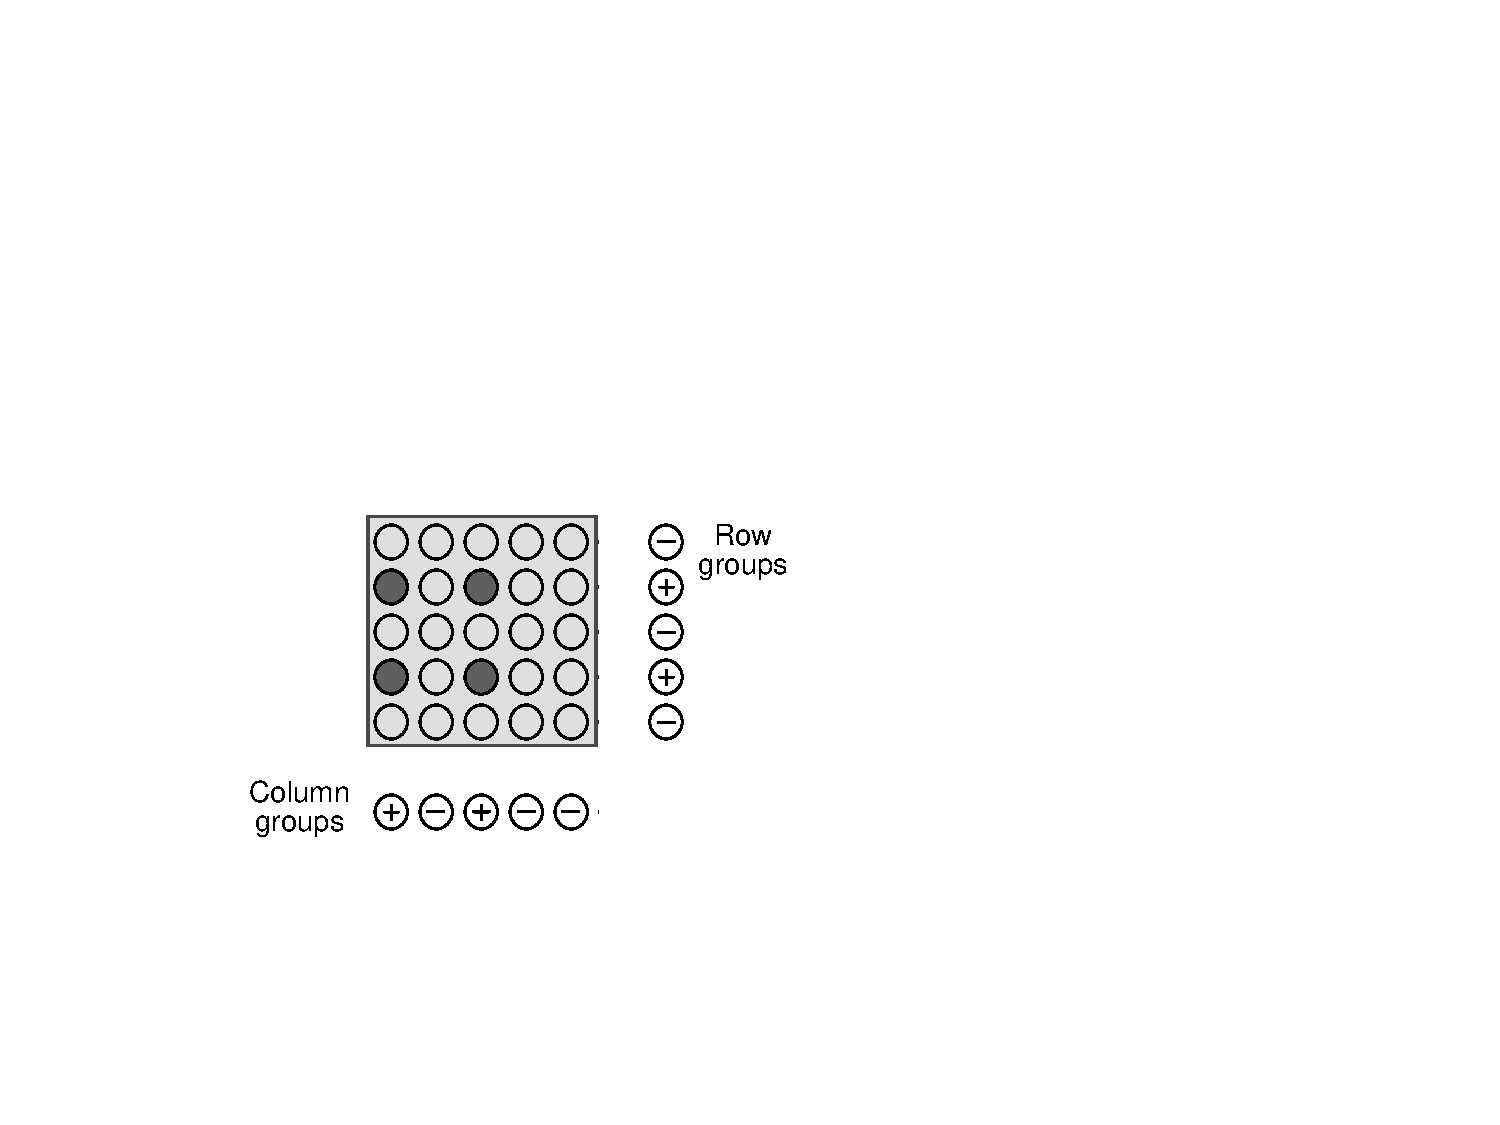
\includegraphics[scale=0.7]{figures/images_array5x5BW.pdf}
\par\end{centering}
\caption{\label{fig:array-1-1}The array testing algorithm of \citet{LabCorp}.
Circles within the square represent specimen locations. Row and column
groups are formed from the specimens with two each testing positive.
The intersections of these positive rows and columns indicate which
specimens need to be retested (filled-in circles). }
\end{figure}

Array testing has a number of variants in application. For example,
a master group containing portions of all specimens within an array
can be tested first. If this master group is negative, all individuals
are quickly declared negative. If the master group is positive, row
and column groups are tested as usual.

\subsection{Additional considerations}

The probability an individual has an infection plays a very important
role in determining the number of tests needed by any group testing
algorithm. For a homogeneous population of individuals tested, we
can define $p$ as this probability. Equivalently, this $p$ is the
overall infection prevalence. In general, the lower (higher) the $p$,
the lower (higher) the expected number of tests needed for group testing
(see e.g. Figure 3 of \citet{Kim2007} and Table 1 of \citet{bilder2021pool}).

In many situations, additional information is available on each individual
to be tested. This information can be used to determine an individual-specific
probability of an infection, say $p_{i}$, which can be incorporated
into the group testing algorithm to reduce the number of tests (\citealt{Bilder2010b};
\citealt{lewis2012cost}). For example, testing is performed by public
health laboratories across the United States for \emph{Chlamydia trachomatis}
(CT) and \emph{Neisseria gonorrhoeae} (NG), the bacteria that lead
to chlamydia and gonorrhea, respectively. Clinics collecting specimens
also obtain important information on their patients, including recent
sexual history and whether a patient has symptoms, and this information
can be incorporated into a statistical model to estimate individual-specific
probabilities of infection. In general, group testing algorithms that
take advantage of this type of additional information are referred
to as being ``informative'' hierarchical/non-hierarchical algorithms
(\citealt{mcmahan2012informative}; \citealt{mcmahan2012two}).

Group testing algorithms can also be used with multiplex assays. Thus,
rather than testing for only one infection, multiple infections can
be detected simultaneously. For example, Roche was the first to receive
an Emergency Use Authorization for their SARS-CoV-2 and influenza
multiplex assay (\citealt{Roche}). Also, the widely adopted Aptima
Combo 2 Assay (\citealt{Aptima}) is used for CT and NG detection
via group testing. Algorithms with multiplex assays are implemented
in the same way as for single-infection assays, but now a group that
tests positive for \emph{at least one} infection leads to retesting
for \emph{all} infections in the next stage. For example, if a group
tests positive for CT and negative for NG in a two-stage hierarchical
algorithm, each group member is retested for both bacteria in the
second stage. Testing is performed in this manner, rather than retesting
for CT only, because of the dedicated testing platforms used. 

\section[Identification]{Identification\label{sec:Identification}}

Identifying infected individuals is most often the primary goal of
infectious disease testing. Prior to implementing a particular group
testing algorithm for this purpose, laboratories need to know the
expected number of tests. This information is used for planning purposes
to make sure enough resources and staff are available to implement
testing. Because cost is often directly proportional to the number
of tests, the expected number of tests can be used for budgeting purposes
as well.

Define $T$ as the number of tests required to determine the positive/negative
outcomes for $I$ individuals. These $I$ individuals may be those
represented within one initial group for hierarchical testing or in
one array for array testing. For the simplest algorithm, two-stage
hierarchical testing, suppose a single-infection assay is applied
to a homogeneous population. The expected number of tests is
\begin{align*}
E(T) & =1+I\left[S_{e}^{(1)}+(1-S_{p}^{(1)}-S_{e}^{(1)})(1-p)^{I}\right],
\end{align*}

\noindent where $S_{e}^{(1)}$ and $S_{p}^{(1)}$ are the first-stage
sensitivity and specificity, respectively, of the assay. This expression
includes a leading 1 because a single group test starts the testing
process. The $I$ outside of the square brackets is for the separate
tests performed on each individual when the group tests positive (which
has the probability given within the square brackets; see \citet{Kim2007}
and \citet{bilder2019id}). Expressions for $E(T)$ become much more
complicated with other group testing algorithms. This is especially
the case for informative algorithms and when multiplex assays are
used. We refer interested readers to the works of \citet{Kim2007},
\citet{mcmahan2012informative}, \citet{mcmahan2012informative},
\citet{black2015optimal}, \citet{bilder2019informative}, and \citet{houarray1}
for specific expressions and calculation details.

The efficiency of a group testing algorithm is expressed typically
as the expected number of tests per individual $E(T)/I$, rather than
$E(T)$ alone, so that comparisons can be made for different $I$.
 The optimal testing configuration (OTC) is the group size or set
of group sizes needed by a single algorithm to minimize $E(T)/I$.
This testing configuration represents the most efficient process to
implement group testing. In other words, it is the group size(s) that
increases a laboratory's testing capacity to its fullest potential,
because resources saved from its application can be used to test more
specimens by the same algorithm. Unfortunately, closed form expressions
for the OTC do not exist, but grid searches are sufficient to find
it. Note that group testing is more efficient than initially testing
each individual separately when $E(T)/I$<1. This is simply because
testing each individual separately results in 1 test per individual. 

Accuracy is also important to examine for group testing algorithms.
This includes the pooling sensitivity, the probability a truly positive
individual is found to be positive from the group testing algorithm,
and the pooling specificity, the probability a truly negative individual
is found to be negative from the group testing algorithm. These probabilities
are not necessarily equal to an assay's stated sensitivity and specificity
because individuals are tested in one or more groups. For example,
the pooling sensitivity for a two-stage hierarchical algorithm can
be shown to be $S_{e}^{(1)}S_{e}^{(2)}$, where $S_{e}^{(2)}$ is
the sensitivity of the assay at the second stage (\citealt{johnson1991inspection},
\citealt{Kim2007}, and \citealt{hitt2020group1}). Expressions for
these accuracy measures corresponding to other algorithms are available
in the previously mentioned references for $E(T)$. 

One issue related to accuracy is what is known as the \emph{dilution
effect} that sometimes can reduce the sensitivity of a group test.
If the same sample volume is used for a group and individual
test, the dilution effect can occur because each individual is represented
by a smaller portion in the group than if each individual was tested
separately. For example, \citet{abdalhamid2020assessment} used a
sample volume of $250\textrm{\ensuremath{\mu}L}$ for a group of size
5 with each individual contributing $50\textrm{\ensuremath{\mu}L}$.
In their validation study, specimens were tested one at a time using
a sample volume of $250\textrm{\ensuremath{\mu}L}$. Thus, there can
be less pathogen present for the test performed upon the group than
for a test performed upon a single specimen. \citet{bilder2021discussion}
discussed the potential dilution effect and solutions for it. In summary,
the resulting outcome from the dilution effect is often known for
assays (\citealt{tan2020considerations}), like for those using real-time
reverse transcription polymerase chain reaction (RT-qPCR) which was
widely used for SARS-CoV-2 testing. This effect can be accounted for
by specifying a smaller value for a group test sensitivity when computing
$E(T)$. Alternatively, the process for applying the assay can be
changed so that there is not a reduction in the sensitivity (\citealt{abdalhamid2020assessment},
\citealt{sanghani2021concentrating}).

\subsection{Main functions}

There are two main sets of functions in \CRANpkg{binGroup2} used for
identification. First, the \code{opChar1()} and \code{opChar2()}
functions calculate operating characteristics for a group testing
algorithm. These functions are for single-infection and two-infection
assays, where the number in the name designates the number of infections.
Calculations for three or more infection assays are discussed in the
concluding section of the paper. The syntax for \code{opChar1()}
is 

\begin{Schunk}
\begin{Sinput}
opChar1(algorithm, p = NULL, probabilities = NULL, Se = 0.99,
    Sp = 0.99, hier.config = NULL, rowcol.sz = NULL, alpha = 2,
    a = NULL, print.time = TRUE, ...)
\end{Sinput}
\end{Schunk}

\noindent \texttt{}The required \code{algorithm} argument specifies
the chosen group testing algorithm. Possible values for this argument
are listed in Table \ref{tab:Values-for-algorithm}. For example,
a value of \code{"D2"} indicates two-stage hierarchical testing in
a homogeneous population (the ``D'' is for its originator, Robert
Dorfman). The remaining arguments are dependent on the algorithm chosen
or are optional. To indicate the probability of an infection, a scalar
can be given for \code{p} or a vector of potentially different
probabilities for each individual can be given for \code{probabilities}. Rather than
providing a specific vector of probabilities, the \code{p} and \code{alpha}
arguments can be used together for informative group testing algorithms
to specify a beta distribution from which the expected values of order
statistics are found. For this case, \code{p} represents the expected
value of a beta random variable and \code{alpha} represents a shape
parameter. This type of specification is helpful when probabilities
of infection can be characterized well by a beta distribution.

\begin{table}
\caption{\label{tab:Values-for-algorithm}Values for \code{algorithm} in \code{opChar1()}
and \code{opChar2()}. A five-stage informative hierarchical algorithm
(\code{ID5}) is also available for two infections. Informative array
testing is not included for \code{opChar2()} because closed-form
expressions of operating characteristics have not been proposed in
the literature. }

\medskip{}

\centering{}%
\begin{tabular}{cc}
\hline 
\code{algorithm} &
Description\tabularnewline
\hline 
\code{A2} &
Array testing\tabularnewline
\code{A2M} &
Array testing with master group\tabularnewline
\code{D2} &
Two-stage hierarchical\tabularnewline
\code{D3} &
Three-stage hierarchical\tabularnewline
\code{D4} &
Four-stage hierarchical\tabularnewline
\code{IA2} &
Informative array testing\tabularnewline
\code{ID2} &
Two-stage, informative hierarchical\tabularnewline
\code{ID3} &
Three-stage, informative hierarchical\tabularnewline
\code{ID4} &
Four-stage, informative hierarchical\tabularnewline
\hline 
\end{tabular}
\end{table}

For hierarchical algorithms, a group membership matrix (\citealt{bilder2019informative})
must be provided for \code{hier.config} to detail the testing of
each individual. In this matrix, the rows correspond to the stages
of testing, the columns correspond to each individual to be tested,
and the cell values specify the group number of each individual at
each stage. We provide an example of its use shortly. For non-hierarchical
algorithms, the \code{rowcol.sz} argument must be provided for the
row and column size of a square array.

Additional arguments include \code{Se} and \code{Sp} for the sensitivity
and specificity of the assay, respectively. If a single value is given
for one of these arguments, this value is used for each stage. Otherwise,
a vector of values can be given in order of stage. The \texttt{a}
argument specifies individuals for which to compute accuracy measures.
By default, accuracy measures are computed for all individuals. Finally,
\code{print.time} allows users to turn off information regarding
the duration of calculations.

The \code{opChar2()} function follows a similar syntax so we do not
provide it here. The main difference involves \code{p} becoming a
vector of joint probabilities of infection. For example, \code{p = (0.90, 0.03, 0.02, 0.05)}
represents $(p_{--},p_{+-},p_{-+},p_{++})$, where $p_{ab}$ is the
probability of being positive/negative ($+/-$) for infections $a$
and $b$. Also, the \code{probabilities} argument value becomes a
$4\times I$ matrix of these probabilities. Similarly, the \code{alpha}
argument becomes the parameter vector for a Dirichlet distribution.

The second set of functions are \code{OTC1()} and \code{OTC2()}
that find the OTC corresponding to single-infection and two-infection
assays, respectively. The syntax for \code{OTC1()} is

\noindent 

\begin{Schunk}
\begin{Sinput}
OTC1(algorithm, p = NULL, probabilities = NULL, Se = 0.99, Sp = 0.99,
    group.sz, obj.fn = "ET", weights = NULL, alpha = 2, trace = TRUE,
    print.time = TRUE, ...)
\end{Sinput}
\end{Schunk}

\noindent \texttt{}The syntax is similar to \code{opChar1()} as
well, so we highlight the main differences only. There is no group
membership matrix or row/column size specified because \code{OTC1()}
searches for the OTC. Instead, the \code{group.sz} argument specifies
the initial group sizes to search over. For example, a value of \code{3:10}
searches over initial group sizes of 3 to 10 for hierarchical testing
or array testing (row/column size).

The \code{obj.fn} argument of \code{OTC1()} indicates which objective
function to minimize when searching for the OTC. Earlier in this section,
we focused on using the expected number of tests per individual as
this objective function (\code{obj.fn = "ET"}). While this is used
most often in practice, other objective functions are possible (\citealt{hitt2019objective}).
For example, \citet{Graff1972} proposed to minimize a linear combination
of the expected number of tests and the number of misclassified individuals
(false positives, false negatives). This objective function is specified
using \code{"GR"}, and the coefficients in this linear combination
are given in the \code{weights} argument.

The \code{OTC2()} function follows a similar syntax as \code{OTC1()}
with changes like those for \code{opChar2()} compared to \code{opChar1()}.
We next provide examples using these functions for group testing applications.

\subsection[Operating characteristics]{Operating characteristics\label{subsec:Operating-characteristics}}

We illustrate the use of \code{opChar1()} for the three-stage hierarchical
testing algorithm of \citet{lohse2020pooling}. The group membership
matrix for this application is the $3\times30$ matrix below.

\noindent 

\begin{Schunk}
\begin{Sinput}
> group.member <- matrix(data = c(rep(1, times = 30), rep(1:3, each = 10),
     1:30), nrow = 3, ncol = 30, byrow = TRUE)
> group.member[, 11]
\end{Sinput}
\begin{Soutput}
[1]  1  2 11
\end{Soutput}
\end{Schunk}

\noindent 

\noindent For example, the 11th individual is tested initially in
a group of size 30 that includes every specimen (one group overall).
In the second stage, this individual is tested in the second sub-group
of 10 individuals if its first-stage group is positive. In the third
stage, this individual is tested separately if its second-stage group
is positive.

We need to specify $p$ or $p_{i}$ for each individual. In actual
practice, these values will be unknown. However, very good point estimates
are usually available from past testing results in high volume clinical
specimen settings where group testing is used. For the \citet{lohse2020pooling}
application, the observed prevalence of SARS-CoV-2 was 0.0193, so
we use this value here for $p$. By specifying \code{"D3"} for \code{algorithm}
to represent three-stage hierarchical testing, we invoke \code{opChar1()}
as follows.

\noindent 

\begin{Schunk}
\begin{Sinput}
> library(package = "binGroup2")
> save.Lohse <- opChar1(algorithm = "D3", p = 0.0193, Se = 1, Sp = 1,
     hier.config = group.member, print.time = FALSE)
> summary(save.Lohse)
\end{Sinput}
\begin{Soutput}

Algorithm: Non-informative three-stage hierarchical testing 

Testing configuration:
Stage 1: 30
Stage 2: 10,10,10

Expected number of tests: 7.64
Expected number of tests per individual: 0.2547

Accuracy for individuals:
     PSe    PSp   PPPV   PNPV Individuals
1 1.0000 1.0000 1.0000 1.0000         All

Overall accuracy of the algorithm:
     PSe    PSp   PPPV   PNPV
1 1.0000 1.0000 1.0000 1.0000

PSe denotes the pooling sensitivity.
PSp denotes the pooling specificity.
PPPV denotes the pooling positive predictive value.
PNPV denotes the pooling negative predictive value.
\end{Soutput}
\end{Schunk}

\noindent The sensitivity (\code{Se}) and the specificity (\code{Sp})
are set to 1 for each stage because the assay accuracy is not stated
in \citet{lohse2020pooling} or in the product insert of the assay
(\citealt{RealStar}). While the algorithm's accuracy values produced
will not be useful, this approach is often followed in practice to
focus on the expected number of tests regardless of false positives/negatives.

The generic \code{summary()} function uses the corresponding method
function for the class to summarize the operating characteristics.
For example, the expected number of tests per individual is $E(T)/I=0.2547$.
A more compact summary based on the expected number of tests is available
with \code{ExpTests()}.

\begin{Schunk}
\begin{Sinput}
> ExpTests(save.Lohse)
\end{Sinput}
\begin{Soutput}
  ExpTests ExpTestsPerIndividual PercentReductionTests PercentIncreaseTestCap
1   7.6403                0.2547                 74.53                 292.66
\end{Soutput}
\end{Schunk}

\noindent Group testing requires $1-E(T)/I=75\%$ fewer tests on average
than testing each specimen separately. In turn, this leads to a $100\{1/[E(T)/I]-1\}\%=293\%$
increase in testing capacity on average when applying the algorithm
to a continuous stream of specimens. This type of large increase in
testing capacity is why laboratories implemented group testing during
the COVID-19 pandemic.

Our second example focuses on the Aptima Combo 2 Assay and its use
by the State Hygienic Laboratory (SHL) at the University of Iowa.
The SHL tests thousands of female swab specimens each year in groups
of size four using a two-stage hierarchical algorithm. We focus here
instead on their male urine specimens because group testing is not
currently implemented. The reason is due to concern that their infection
prevalence may be too large for group testing to be beneficial. \citet{bilder2019informative}
provided a Dirichlet distribution with parameter vector $\alpha=(10.99,0.18,2.04,0.31)$
to describe a vector of the joint probabilities of infection for CT
and NG that take into account risk factors, such as symptoms and exposure
to an infected individual. Using a first-stage group size of 5, we
want to calculate how well three-stage hierarchical testing would
perform when allowing for differences among probabilities of infection
for individuals. To begin, we simulate what one potential set of
probabilities of infection could be using the Dirichlet distribution
and the \code{rdirichlet()} function of the \CRANpkg{rBeta2009}
package (\citealt{rBeta2009}). These probabilities are ordered by
the probability of having at least one infection.

\begin{Schunk}
\begin{Sinput}
> library(package = "rBeta2009")
> set.seed(3789)
> p.unordered <- t(rdirichlet(n = 5, shape = c(10.99, 0.18, 2.04, 0.31)))
> p.ordered <- p.unordered[, order(1 - p.unordered[1, ])]
> round(p.ordered, 4)
\end{Sinput}
\begin{Soutput}
       [,1]   [,2]   [,3]   [,4]   [,5]
[1,] 0.9714 0.8841 0.8356 0.8291 0.7009
[2,] 0.0001 0.0006 0.0000 0.0238 0.0000
[3,] 0.0274 0.0879 0.1643 0.1292 0.2991
[4,] 0.0011 0.0274 0.0001 0.0178 0.0000
\end{Soutput}
\end{Schunk}

Next, we create the group membership matrix for three-stage informative
hierarchical testing using the OTC found in \citet{bilder2019informative}.
Because individuals 4 and 5 are tested separately in the second stage,
a \code{NA} is used for them in the third stage of the group membership
matrix.

\begin{Schunk}
\begin{Sinput}
> group.member <- matrix(data = c(rep(1, times = 5), 1, 1, 1, 2, 3, 1, 2,
     3, NA, NA), nrow = 3, ncol = 5, byrow = TRUE)
> group.member
\end{Sinput}
\begin{Soutput}
     [,1] [,2] [,3] [,4] [,5]
[1,]    1    1    1    1    1
[2,]    1    1    1    2    3
[3,]    1    2    3   NA   NA
\end{Soutput}
\end{Schunk}

Lastly, the \code{opChar2()} function calculates the operating characteristics
for the algorithm. The \code{Se} and \code{Sp} matrices provide
the sensitivity and specificity values, respectively, for each infection
at each stage (\citealt{IowaComm}). Because these accuracies are
equal across the stages, the sensitivity (specificity) for CT and
NG could be instead included as a single vector of length 2 for the
\code{Se} (\code{Sp}) argument of \code{opChar2()}. Alternatively,
if accuracies were different across stages, the full matrices provide
a general way to include this information.

\begin{Schunk}
\begin{Sinput}
> Se <- matrix(data = rep(c(0.979, 0.985), times = 3), nrow = 2, ncol = 3,
     dimnames = list(Infection = 1:2, Stage = 1:3))
> Sp <- matrix(data = rep(c(0.985, 0.996), times = 3), nrow = 2, ncol = 3,
     dimnames = list(Infection = 1:2, Stage = 1:3))
> save.SHL <- opChar2(algorithm = "ID3", probabilities = p.ordered, Se = Se,
     Sp = Sp, hier.config = group.member, print.time = FALSE)
> summary(save.SHL)
\end{Sinput}
\begin{Soutput}

Algorithm: Informative three-stage hierarchical testing 

Testing configuration:
Stage 1: 5
Stage 2: 3,1,1

Expected number of tests: 3.59
Expected number of tests per individual: 0.7182

Disease 1 accuracy for individuals:
     PSe    PSp   PPPV   PNPV Individuals
1 0.9770 0.9958 0.2111 1.0000           1
2 0.9778 0.9961 0.8784 0.9994           2
3 0.9784 0.9958 0.0124 1.0000           3
4 0.9729 0.9915 0.8330 0.9988           4
5 0.9787 0.9913 0.0012 1.0000           5

Disease 2 accuracy for individuals:
     PSe    PSp   PPPV   PNPV Individuals
1 0.9585 0.9990 0.9643 0.9988           1
2 0.9633 0.9992 0.9940 0.9952           2
3 0.9575 0.9994 0.9969 0.9917           3
4 0.9725 0.9979 0.9879 0.9953           4
5 0.9714 0.9984 0.9961 0.9879           5

Overall accuracy of the algorithm:
     PSe    PSp   PPPV   PNPV
1 0.9749 0.9941 0.7039 0.9996
2 0.9669 0.9988 0.9931 0.9941

PSe denotes the pooling sensitivity.
PSp denotes the pooling specificity.
PPPV denotes the pooling positive predictive value.
PNPV denotes the pooling negative predictive value.
\end{Soutput}
\end{Schunk}

 The expected number of tests per individual is 0.7182. Because
this value is less than 1, group testing would be more efficient on average
than testing each individual separately. The PSe and PSp values in
the output are the pooling sensitivity and specificity, respectively.
Additionally, values are given for the pooling positive predictive
value (PPPV) and the pooling negative predictive value (PNPV; see
\citet{altman1994statistics} and \citet{hitt2019objective}).

Of course, not every set of 5 individuals has these 5 joint probabilities
of infection. When this group testing algorithm was applied to the
data from which the Dirichlet distribution was estimated, \citet{bilder2019informative}
showed that the number of tests decreased by approximately 26\% on
average. 

\subsection[Optimal testing configuration]{Optimal testing configuration\label{subsec:Optimal-testing-configuration}}

Returning to the three-stage hierarchical algorithm of \citet{lohse2020pooling},
suppose again that $p=0.0193$. The OTC is found using the following
code. 

\noindent 

\begin{Schunk}
\begin{Sinput}
> OTC.Lohse <- OTC1(algorithm = "D3", p = 0.0193, Se = 1, Sp = 1,
     group.sz = 3:20, obj.fn = "ET", print.time = FALSE)
\end{Sinput}
\begin{Soutput}
Initial Group Size = 3
Initial Group Size = 4
Initial Group Size = 5
Initial Group Size = 6
Initial Group Size = 7
Initial Group Size = 8
Initial Group Size = 9
Initial Group Size = 10
Initial Group Size = 11
Initial Group Size = 12
Initial Group Size = 13
Initial Group Size = 14
Initial Group Size = 15
Initial Group Size = 16
Initial Group Size = 17
Initial Group Size = 18
Initial Group Size = 19
Initial Group Size = 20
\end{Soutput}
\begin{Sinput}
> summary(OTC.Lohse)
\end{Sinput}
\begin{Soutput}

Algorithm: Non-informative three-stage hierarchical testing 

Optimal testing configuration:
   Stage 1 Stage 2
ET      16 4,4,4,4

Expected number of tests:
   E(T)  Value
ET 3.27 0.2045

E(T) denotes the expected number of tests.
Value denotes the objective function value per individual.

Overall accuracy of the algorithm:
      PSe    PSp   PPPV   PNPV
ET 1.0000 1.0000 1.0000 1.0000

PSe denotes the pooling sensitivity.
PSp denotes the pooling specificity.
PPPV denotes the pooling positive predictive value.
PNPV denotes the pooling negative predictive value.
\end{Soutput}
\end{Schunk}

\noindent The \code{summary()} function summarizes the OTC. The
first-stage group size is 16, the second stage has 4 groups of size
4, and the third stage uses individual testing. The expected number
of tests per individual is 0.2045. Therefore, the OTC decreases the
expected number of tests per individual further by almost 20\% ($=(0.2547-0.2045)/0.2547$)
over the testing configuration used by \citet{lohse2020pooling}.
In terms of expected test capacity, one can show with \code{ExpTests(OTC.Lohse)}
that the OTC leads to a 389\% increase in testing capacity when compared
to testing each specimen separately. Again, this is significantly
better than the testing configuration chosen by \citet{lohse2020pooling}
and helps to show the importance of choosing a testing configuration.

The \code{OTC1()} function searches for the optimal set of group
sizes at \emph{each} first-stage group size specified in the \code{group.sz}
argument. By default, the function's progress is printed during its
running (\code{trace = TRUE}). We take this approach to finding the
OTC, rather than optimizing over all group sizes initially, because
a laboratory may prefer a sub-optimal testing configuration due to
their work environment. The \code{Config()} function provides information
about these sub-optimal testing configurations. This function extracts
each of the best testing configurations by initial group size and
returns them as a data frame sorted by the value of the objective
function ($E(T)/I$ because the default was used in \code{OTC1()}).

\begin{Schunk}
\begin{Sinput}
> Config(OTC.Lohse)
\end{Sinput}
\begin{Soutput}
   I    config     ET  value PSe PSp PPPV PNPV
1 16   4,4,4,4 3.2714 0.2045   1   1    1    1
2 17   5,4,4,4 3.4922 0.2054   1   1    1    1
3 15   4,4,4,3 3.0842 0.2056   1   1    1    1
4 20 4,4,4,4,4 4.1138 0.2057   1   1    1    1
5 19 4,4,4,4,3 3.9176 0.2062   1   1    1    1
\end{Soutput}
\end{Schunk}

\noindent Adding \code{top.overall = TRUE} to \code{Config()} provides
the same information but with the top testing configurations overall
rather than for each initial group size.

The most efficient outcome from the OTC depends on the chosen value
of $p$. As mentioned earlier in this section, very good point estimates
for $p$ are often available. Still, it would be of interest to determine
what would occur for other choices of $p$. The \CRANpkg{binGroup2} package
provides the tools needed by experienced R users for this more in
depth examination. Our Appendix A discusses additional code using
\code{OTC1()} to produce Figure \ref{fig:Expected-number-of}. The
testing configuration chosen by \citet{lohse2020pooling} is never
optimal. In fact, two-stage hierarchical group testing is more efficient
than \citet{lohse2020pooling} for $p>0.03$. 

\begin{figure}
\noindent \begin{centering}
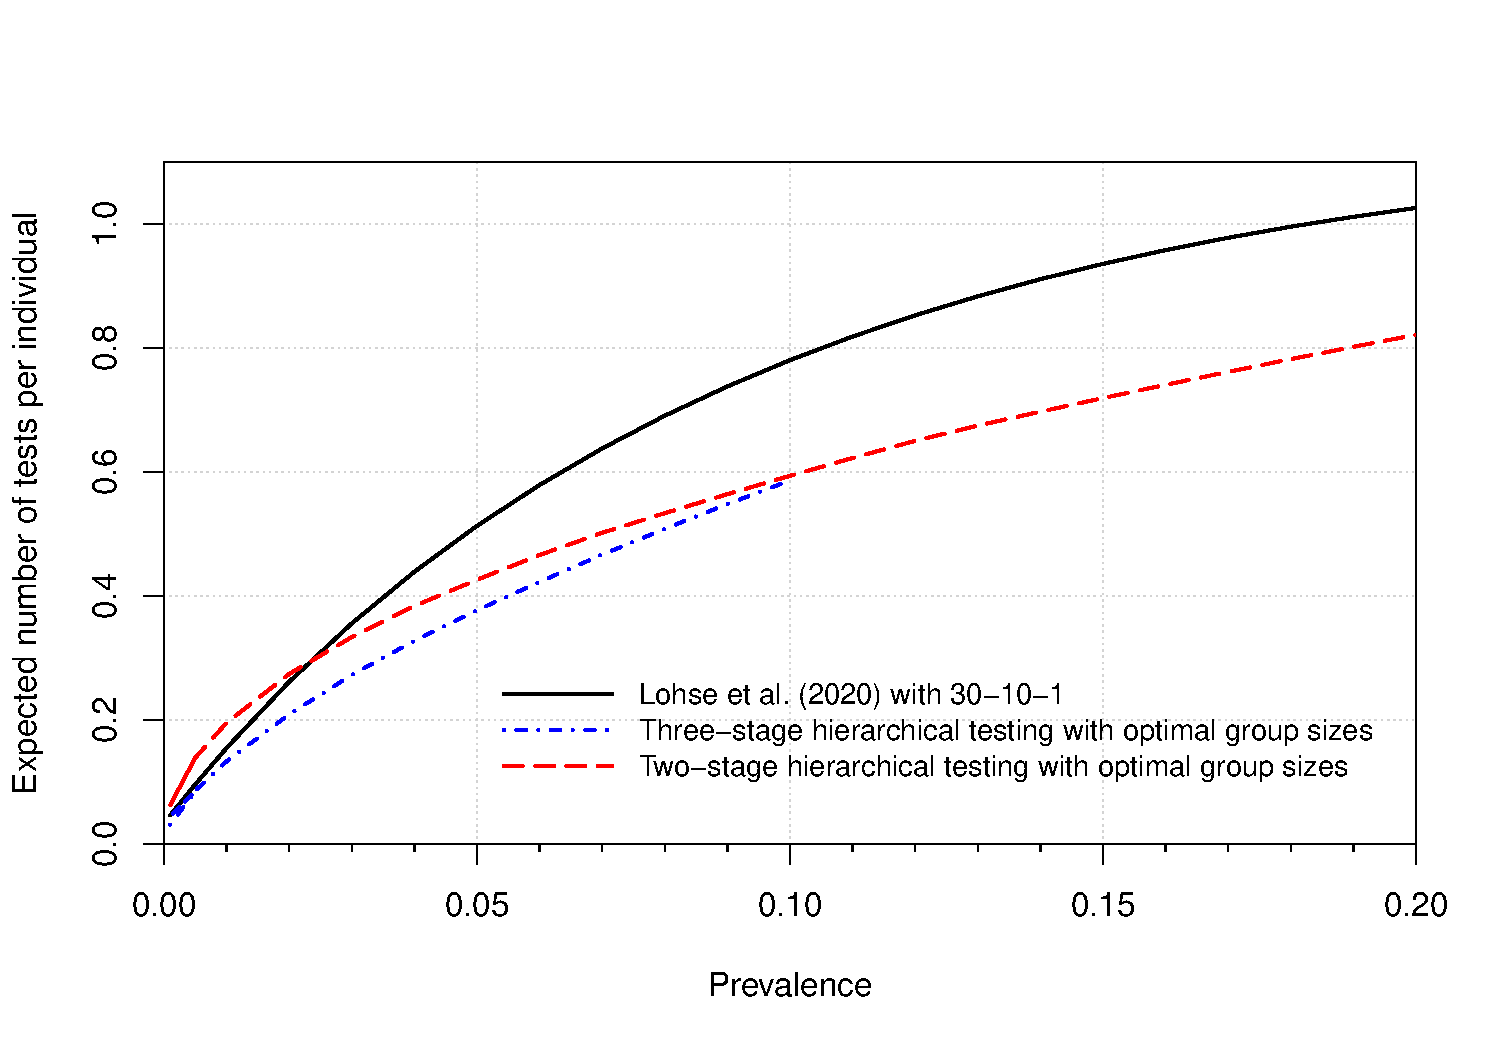
\includegraphics[scale=0.55]{figures/Lohse.pdf}
\par\end{centering}
\caption{Expected number of tests per individual as a function of infection
prevalence. Three-stage hierarchical testing using the OTC is not
plotted for prevalences greater than 0.10 because two stages results
in a lower expected number of tests. \label{fig:Expected-number-of}}
\end{figure}

Our second example focuses on SARS-CoV-2 detection again, but now
in the context of LabCorp's array testing. \citet{LabCorp} examined
the potential performance of their approach using possible prevalences
between 0.001 and 0.15, so we begin with using a prevalence of 0.05.
Also, \citet{LabCorp} estimated that approximately 0.023 of all positives
would be missed using array testing rather than individual testing.
This is not quite the sensitivity of the assay, but we will use 0.977
and 1 as the sensitivity for the first and second stages, respectively,
for illustration purposes. We will also use 1 as the specificity for
illustration purposes. The expected number of tests per individual
for the algorithm is found first using \code{opChar1()} with \code{algorithm = "A2"}.

\noindent 

\begin{Schunk}
\begin{Sinput}
> save.LabCorp <- opChar1(algorithm = "A2", p = 0.05, rowcol.sz = 5,
     Se = c(1 - 0.023, 1), Sp = 1, print.time = FALSE)
> ExpTests(save.LabCorp)
\end{Sinput}
\begin{Soutput}
  ExpTests ExpTestsPerIndividual PercentReductionTests PercentIncreaseTestCap
1  12.0763                0.4831                 51.69                 107.02
\end{Soutput}
\end{Schunk}

\noindent The expected number of tests per individual is 0.48, resulting
in an expected 107\% increase in testing capacity.

Could LabCorp do better? Below is the code used to find the OTC for
a range of group sizes from 3 to 10 with array testing. 

\noindent 

\begin{Schunk}
\begin{Sinput}
> OTC.LabCorp.Array <- OTC1(algorithm = "A2", p = 0.05, Se = c(0.977,
     1), Sp = 1, group.sz = 3:10, obj.fn = "ET", trace = FALSE,
     print.time = FALSE)
> summary(OTC.LabCorp.Array)
\end{Sinput}
\begin{Soutput}

Algorithm: Non-informative array testing without master pooling 

Optimal testing configuration:
   Row/column size Array size
ET              10        100

Expected number of tests:
    E(T)  Value
ET 37.20 0.3720

E(T) denotes the expected number of tests.
Value denotes the objective function value per individual.

Overall accuracy of the algorithm:
      PSe    PSp   PPPV   PNPV
ET 0.9550 1.0000 1.0000 0.9976

PSe denotes the pooling sensitivity.
PSp denotes the pooling specificity.
PPPV denotes the pooling positive predictive value.
PNPV denotes the pooling negative predictive value.
\end{Soutput}
\begin{Sinput}
> ExpTests(OTC.LabCorp.Array)
\end{Sinput}
\begin{Soutput}
       ExpTests ExpTestsPerInd PercentReductionTests PercentIncreaseTestCap
opt.ET  37.1953         0.3720                 62.80                 168.85
\end{Soutput}
\end{Schunk}

The OTC for array testing is a $10\times10$ array that has an expected
number of tests per individual of 0.37 and an increase in testing
capacity of 169\%. This is a significant improvement over the $5\times5$
array. One could perform similar calculations using two-stage hierarchical
testing with \code{algorithm = "D2"} in \code{OTC1}. This results
in an OTC that uses an initial group size of 5 and leads to an expected
number of tests per individual of 0.42. 

Because these calculations rely on $p=0.05$, Appendix B includes
additional results for different values of $p$ and a discussion of
the corresponding more advanced code. In most cases, we find that
a $5\times5$ array is not the OTC. 

\subsection[Additional functions]{Additional functions\label{subsec:Additional functions-1}}

Not all group testing algorithms fit well within a general computing
framework. For this reason, we include a few additional functions
outside of those discussed previously. In particular, the \code{halving()}
and \code{Sterrett()} functions provide alternative ways to use hierarchical
testing algorithms. The former function calculates operating characteristics
when positive testing groups are split only in half (\citealt{litvak1994screening};
\citealt{black2012group}). The latter function calculates operating
characteristics for algorithms that retest only one specimen at a
time from a positive group (\citealt{sterrett1957detection}; \citealt{Bilder2010a}).
Once a positive is found, the remaining specimens are retested again
in a group. The idea behind this strategy is there will likely be
only one positive (or few positives) in the original group. 


\section[Conclusion]{Conclusion\label{sec:Conclusion}}

The \CRANpkg{binGroup2} package provides researchers and laboratories
with the statistical tools needed to implement group testing 
effectively. An earlier version of this package was used as well
by \emph{The New York Times} to help readers understand the benefits
from group testing during the COVID-19 pandemic (\citealt{NYTimesBui}).
Similar to \citet{Bilder2010b}, we encourage researchers to submit
their own functions to us to be included within the package. This
will allow users to have one overall package rather than many packages
that may duplicate the work of others. 

The identification functions are for one and two-infection assays.
While there are a few three- and four-infection assays for infectious
disease detection that have been recently released (e.g., the BD Max
CT/GC/TV assay (\citealt{BD}) that tests for pathogens which lead
to chlamydia, gonorrhea, and trichomoniasis), these assays are used
currently much less than single and two-infection assays. Also, derivations
for operating characteristics become much more complex for more than
two infections, so there are no closed-form expressions available
for these types of assays. For example, \citet{houarray1} needed
Monte Carlo simulation for a three-infection assay. We anticipate
that it will be useful to include Monte Carlo simulation-based estimates
of operating characteristics in future versions of \CRANpkg{binGroup2}
as these types of multiplex assays become more widely used. New research
is needed though to find efficient computational approaches when searching
for the OTC because of these simulation aspects.

While not the focus of this paper, the estimation functions from \CRANpkg{binGroup}
have been simplified and expanded upon using a coherent style. The
new \code{propCI()} function combines three previous functions into
one to calculate point estimates and confidence intervals for an infection
prevalence. The new \code{propDiffCI()} provides similar functionality
for the difference of two infection prevalences. Both functions incorporate
new research since \citet{Bilder2010b}. In particular, the bias correction
methods of \citet{hepworth2017bias} are included to account for the
long-standing problem of bias for point estimates in group testing
(\citealt{swallow1985group}). The \code{gtReg()} function combines
three previous \CRANpkg{binGroup} functions used to estimate regression
models with group testing data that arise from different testing algorithms.
The \code{gtSim()} function also combines three previous \CRANpkg{binGroup}
functions to simulate group testing data with covariates that can
arise from different testing algorithms.

\section{Acknowledgments}

The authors thank Jeffrey Benfer and Kristopher Eveland at the SHL
and Peter Iwen and Baha Abdalhamid at the Nebraska Public Health Laboratory
for their consultation on CT/NG and SARS-CoV-2 testing. This research
was supported by Grant R01 AI121351 from the National Institutes of
Health. The views expressed in this article are those of the authors
and do not necessarily reflect the official policy or position of
the United States Air Force Academy, the Air Force, the Department
of Defense, or the U.S. Government. Approved for public release: distribution
unlimited. PA\#: USAFA-DF-2022-474.

%Appendix A: Details for Figure \ref{fig:Expected-number-of}
\section{Appendix A: Details for figure}

Our separate R program provides the code to create Figure \ref{fig:Expected-number-of}.
This figure presents a comparison of the three-stage hierarchical
testing algorithm of \citet{lohse2020pooling} to using the OTC for
two- and three-stage hierarchical testing. We use the \code{OTC1()}
function to find the OTCs for the prevalences of 0.001, 0.005, and
0.01 to 0.20 by 0.01 with a maximum group size of 64. The large number
of prevalences and large group sizes will result in a significant
amount of computational time. For readers interested in testing the
code, we recommend using a few prevalence values and a maximum group
size of 30 for an initial running of it. 

% Appendix B: LabCorp's Array Testing
\section{Appendix B: Labcorp's array testing}

\citet{LabCorp} described the use of arrays for up to size $5\times5$.
Our separate R program provides the code  to create Figure \ref{fig:LabCorp}
that examines their use further. This figure  provides evidence that
a $5\times5$ array size is not an optimal choice. For the corresponding
calculations, we found the OTC for array testing by minimizing the
expected number of tests per individual for the prevalences of 0.001,
0.005, and 0.01 to 0.20 by 0.01. Because two-stage hierarchical testing
is also frequently used for SARS-CoV-2 detection, we also found the
OTC for this algorithm. Throughout these calculations, we conservatively
limit the maximum group size to 10. 

\begin{figure}
\noindent \begin{centering}
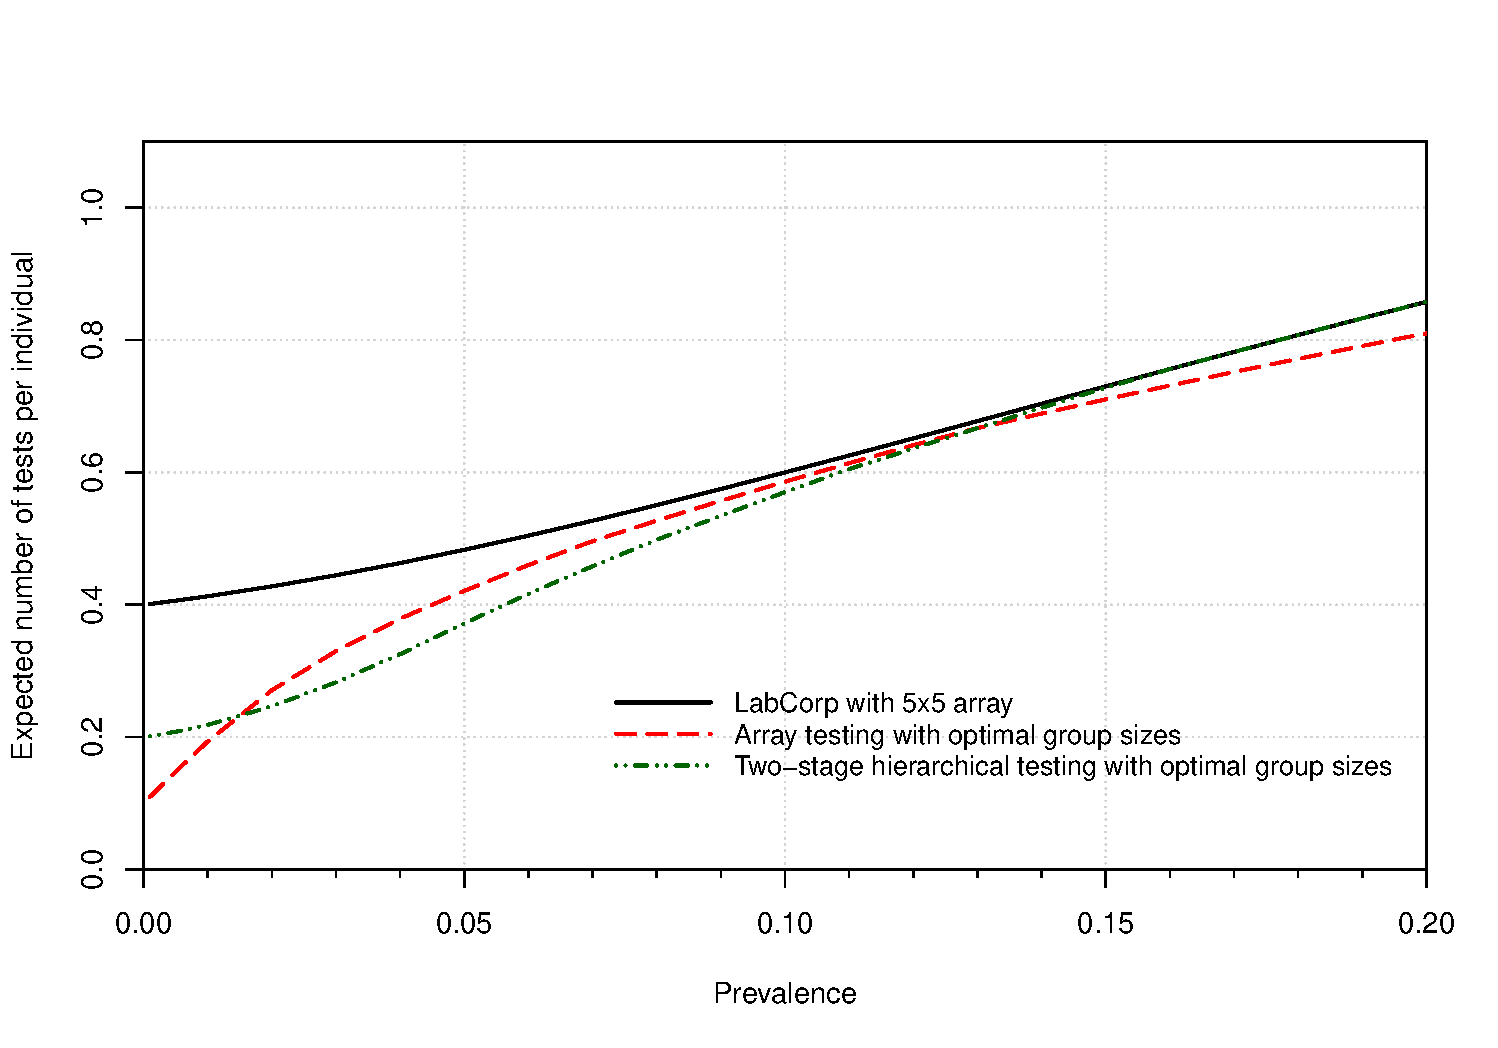
\includegraphics[scale=0.55]{figures/LabCorp.pdf}
\par\end{centering}
\caption{Expected number of tests per individual as a function of infection
prevalence for LabCorp's setting. \label{fig:LabCorp}}
\end{figure}



\hypertarget{refs}{}

\bibliography{refs.bib}

\address{%
Christopher R. Bilder\\
University of Nebraska-Lincoln\\%
Department of Statistics\\ Lincoln, NE 68583, USA\\ \url{www.chrisbilder.com}\\
%
%
%
\href{mailto:chris@chrisbilder.com}{\nolinkurl{chris@chrisbilder.com}}%
}

\address{%
Brianna D. Hitt\\
United States Air Force Academy\\%
Department of Mathematical Sciences\\ Colorado Springs, CO 80840, USA\\
%
%
%
\href{mailto:brianna.hitt@afacademy.af.edu}{\nolinkurl{brianna.hitt@afacademy.af.edu}}%
}

\address{%
Brad J. Biggerstaff\\
Centers for Disease Control and Prevention\\%
Division of Vector-Borne Diseases\\ Fort Collins, CO 80521, USA\\
%
%
%
\href{mailto:bkb5@cdc.gov}{\nolinkurl{bkb5@cdc.gov}}%
}

\address{%
Joshua M. Tebbs\\
University of South Carolina\\%
Department of Statistics\\ Columbia, SC 29208, USA\\
%
%
%
\href{mailto:tebbs@stat.sc.edu}{\nolinkurl{tebbs@stat.sc.edu}}%
}

\address{%
Christopher S. McMahan\\
Clemson University\\%
School of Mathematical and Statistical Sciences\\ Clemson, SC 29634, USA\\
%
%
%
\href{mailto:mcmaha2@clemson.edu}{\nolinkurl{mcmaha2@clemson.edu}}%
}
